\documentclass[14pt,russian]{scrartcl}
\let\counterwithout\relax
\let\counterwithin\relax
\usepackage{lmodern}
\usepackage{float}
\usepackage{xcolor}
\usepackage{extsizes}
\usepackage{subfig}
\usepackage[export]{adjustbox}
\usepackage{tocvsec2} % возможность менять учитываемую глубину разделов в оглавлении
\usepackage[subfigure]{tocloft}

\usepackage{fancyvrb}
\usepackage{ulem,bm,mathrsfs,ifsym} %зачеркивания, особо жирный стиль и RSFS начертание
\usepackage{sectsty} % переопределение стилей подразделов
%%%%%%%%%%%%%%%%%%%%%%%

%%% Поля и разметка страницы %%%
\usepackage{pdflscape}                              % Для включения альбомных страниц
\usepackage{geometry}                               % Для последующего задания полей
\geometry{a4paper,tmargin=2cm,bmargin=2cm,lmargin=3cm,rmargin=1cm} % тоже самое, но лучше

%%% Математические пакеты %%%
\usepackage{amsthm,amsfonts,amsmath,amssymb,amscd}  % Математические дополнения от AMS
\usepackage{mathtools}                              % Добавляет окружение multlined
\usepackage[perpage]{footmisc}

%%%% Установки для размера шрифта 14 pt %%%%
%% Формирование переменных и констант для сравнения (один раз для всех подключаемых файлов)%%
%% должно располагаться до вызова пакета fontspec или polyglossia, потому что они сбивают его работу
%\newlength{\curtextsize}
%\newlength{\bigtextsize}
%\setlength{\bigtextsize}{13pt}
\KOMAoptions{fontsize=14pt}

\makeatletter
\def\showfontsize{\f@size{} point}
\makeatother

%\makeatletter
%\show\f@size                                       % неплохо для отслеживания, но вызывает стопорение процесса, если документ компилируется без команды  -interaction=nonstopmode 
%\setlength{\curtextsize}{\f@size pt}
%\makeatother

%шрифт times
\usepackage{tempora}

   %%% Решение проблемы копирования текста в буфер кракозябрами
%    \input glyphtounicode.tex
%    \input glyphtounicode-cmr.tex %from pdfx package
%    \pdfgentounicode=1
    \usepackage{cmap}                               % Улучшенный поиск русских слов в полученном pdf-файле
    \usepackage[T2A]{fontenc}                       % Поддержка русских букв
    \usepackage[utf8]{inputenc}                     % Кодировка utf8
    \usepackage[english, main=russian]{babel}            % Языки: русский, английский
%   \IfFileExists{pscyr.sty}{\usepackage{pscyr}}{}  % Красивые русские шрифты
%\renewcommand{\rmdefault}{ftm}
%%% Оформление абзацев %%%
\usepackage{indentfirst}                            % Красная строка
%\usepackage{eskdpz}

%%% Таблицы %%%
\usepackage{longtable}                              % Длинные таблицы
\usepackage{multirow,makecell,array}                % Улучшенное форматирование таблиц
\usepackage{booktabs}                               % Возможность оформления таблиц в классическом книжном стиле (при правильном использовании не противоречит ГОСТ)

%%% Общее форматирование
\usepackage{soulutf8}                               % Поддержка переносоустойчивых подчёркиваний и зачёркиваний
\usepackage{icomma}                                 % Запятая в десятичных дробях



%%% Изображения %%%
\usepackage{graphicx}                               % Подключаем пакет работы с графикой
\usepackage{wrapfig}

%%% Списки %%%
\usepackage{enumitem}

%%% Подписи %%%
\usepackage{caption}                                % Для управления подписями (рисунков и таблиц) % Может управлять номерами рисунков и таблиц с caption %Иногда может управлять заголовками в списках рисунков и таблиц
%% Использование:
%\begin{table}[h!]\ContinuedFloat - чтобы не переключать счетчик
%\captionsetup{labelformat=continued}% должен стоять до самого caption
%\caption{}
% либо ручками \caption*{Продолжение таблицы~\ref{...}.} :)

%%% Интервалы %%%

%%% Счётчики %%%
\usepackage[figure,table,section]{totalcount}               % Счётчик рисунков и таблиц
\DeclareTotalCounter{lstlisting}
\usepackage{totcount}                               % Пакет создания счётчиков на основе последнего номера подсчитываемого элемента (может требовать дважды компилировать документ)
\usepackage{totpages}                               % Счётчик страниц, совместимый с hyperref (ссылается на номер последней страницы). Желательно ставить последним пакетом в преамбуле

%%% Продвинутое управление групповыми ссылками (пока только формулами) %%%
%% Кодировки и шрифты %%%

%   \newfontfamily{\cyrillicfont}{Times New Roman}
%   \newfontfamily{\cyrillicfonttt}{CMU Typewriter Text}
	%\setmainfont{Times New Roman}
	%\newfontfamily\cyrillicfont{Times New Roman}
	%\setsansfont{Times New Roman}                    %% задаёт шрифт без засечек
%	\setmonofont{Liberation Mono}               %% задаёт моноширинный шрифт
 %   \IfFileExists{pscyr.sty}{\renewcommand{\rmdefault}{ftm}}{}
%%% Интервалы %%%
%linespread-реализация ближе к реализации полуторного интервала в ворде.
%setspace реализация заточена под шрифты 10, 11, 12pt, под остальные кегли хуже, но всё же ближе к типографской классике. 
\linespread{1.3}                    % Полуторный интервал (ГОСТ Р 7.0.11-2011, 5.3.6)
%\renewcommand{\@biblabel}[1]{#1}

%%% Гиперссылки %%%
\usepackage{hyperref}

%%% Выравнивание и переносы %%%
\sloppy                             % Избавляемся от переполнений
\clubpenalty=10000                  % Запрещаем разрыв страницы после первой строки абзаца
\widowpenalty=10000                 % Запрещаем разрыв страницы после последней строки абзаца

\makeatletter % малые заглавные, small caps shape
\let\@@scshape=\scshape
\renewcommand{\scshape}{%
  \ifnum\strcmp{\f@series}{bx}=\z@
    \usefont{T1}{cmr}{bx}{sc}%
  \else
    \ifnum\strcmp{\f@shape}{it}=\z@
      \fontshape{scsl}\selectfont
    \else
      \@@scshape
    \fi
  \fi}
\makeatother

%%% Подписи %%%
%\captionsetup{%
%singlelinecheck=off,                % Многострочные подписи, например у таблиц
%skip=2pt,                           % Вертикальная отбивка между подписью и содержимым рисунка или таблицы определяется ключом
%justification=centering,            % Центрирование подписей, заданных командой \caption
%}
%%%        Подключение пакетов                 %%%
\usepackage{ifthen}                 % добавляет ifthenelse
%%% Инициализирование переменных, не трогать!  %%%
\newcounter{intvl}
\newcounter{otstup}
\newcounter{contnumeq}
\newcounter{contnumfig}
\newcounter{contnumtab}
\newcounter{pgnum}
\newcounter{bibliosel}
\newcounter{chapstyle}
\newcounter{headingdelim}
\newcounter{headingalign}
\newcounter{headingsize}
\newcounter{tabcap}
\newcounter{tablaba}
\newcounter{tabtita}
%%%%%%%%%%%%%%%%%%%%%%%%%%%%%%%%%%%%%%%%%%%%%%%%%%

%%% Область упрощённого управления оформлением %%%

%% Интервал между заголовками и между заголовком и текстом
% Заголовки отделяют от текста сверху и снизу тремя интервалами (ГОСТ Р 7.0.11-2011, 5.3.5)
\setcounter{intvl}{3}               % Коэффициент кратности к размеру шрифта

%% Отступы у заголовков в тексте
\setcounter{otstup}{0}              % 0 --- без отступа; 1 --- абзацный отступ

%% Нумерация формул, таблиц и рисунков
\setcounter{contnumeq}{1}           % Нумерация формул: 0 --- пораздельно (во введении подряд, без номера раздела); 1 --- сквозная нумерация по всей диссертации
\setcounter{contnumfig}{1}          % Нумерация рисунков: 0 --- пораздельно (во введении подряд, без номера раздела); 1 --- сквозная нумерация по всей диссертации
\setcounter{contnumtab}{1}          % Нумерация таблиц: 0 --- пораздельно (во введении подряд, без номера раздела); 1 --- сквозная нумерация по всей диссертации

%% Оглавление
\setcounter{pgnum}{0}               % 0 --- номера страниц никак не обозначены; 1 --- Стр. над номерами страниц (дважды компилировать после изменения)

%% Библиография
\setcounter{bibliosel}{1}           % 0 --- встроенная реализация с загрузкой файла через движок bibtex8; 1 --- реализация пакетом biblatex через движок biber

%% Текст и форматирование заголовков
\setcounter{chapstyle}{1}           % 0 --- разделы только под номером; 1 --- разделы с названием "Глава" перед номером
\setcounter{headingdelim}{1}        % 0 --- номер отделен пропуском в 1em или \quad; 1 --- номера разделов и приложений отделены точкой с пробелом, подразделы пропуском без точки; 2 --- номера разделов, подразделов и приложений отделены точкой с пробелом.

%% Выравнивание заголовков в тексте
\setcounter{headingalign}{0}        % 0 --- по центру; 1 --- по левому краю

%% Размеры заголовков в тексте
\setcounter{headingsize}{0}         % 0 --- по ГОСТ, все всегда 14 пт; 1 --- пропорционально изменяющийся размер в зависимости от базового шрифта

%% Подпись таблиц
\setcounter{tabcap}{0}              % 0 --- по ГОСТ, номер таблицы и название разделены тире, выровнены по левому краю, при необходимости на нескольких строках; 1 --- подпись таблицы не по ГОСТ, на двух и более строках, дальнейшие настройки: 
%Выравнивание первой строки, с подписью и номером
\setcounter{tablaba}{2}             % 0 --- по левому краю; 1 --- по центру; 2 --- по правому краю
%Выравнивание строк с самим названием таблицы
\setcounter{tabtita}{1}             % 0 --- по левому краю; 1 --- по центру; 2 --- по правому краю

%%% Рисунки %%%
\DeclareCaptionLabelSeparator*{emdash}{~--- }             % (ГОСТ 2.105, 4.3.1)
\captionsetup[figure]{labelsep=emdash,font=onehalfspacing,position=bottom}

\captionsetup[lstlisting]{justification=raggedright, singlelinecheck=false}

%%% Таблицы %%%
\ifthenelse{\equal{\thetabcap}{0}}{%
    \newcommand{\tabcapalign}{\raggedright}  % по левому краю страницы или аналога parbox
}

\ifthenelse{\equal{\thetablaba}{0} \AND \equal{\thetabcap}{1}}{%
    \newcommand{\tabcapalign}{\raggedright}  % по левому краю страницы или аналога parbox
}

\ifthenelse{\equal{\thetablaba}{1} \AND \equal{\thetabcap}{1}}{%
    \newcommand{\tabcapalign}{\centering}    % по центру страницы или аналога parbox
}

\ifthenelse{\equal{\thetablaba}{2} \AND \equal{\thetabcap}{1}}{%
    \newcommand{\tabcapalign}{\raggedleft}   % по правому краю страницы или аналога parbox
}

\ifthenelse{\equal{\thetabtita}{0} \AND \equal{\thetabcap}{1}}{%
    \newcommand{\tabtitalign}{\raggedright}  % по левому краю страницы или аналога parbox
}

\ifthenelse{\equal{\thetabtita}{1} \AND \equal{\thetabcap}{1}}{%
    \newcommand{\tabtitalign}{\centering}    % по центру страницы или аналога parbox
}

\ifthenelse{\equal{\thetabtita}{2} \AND \equal{\thetabcap}{1}}{%
    \newcommand{\tabtitalign}{\raggedleft}   % по правому краю страницы или аналога parbox
}

\DeclareCaptionFormat{tablenocaption}{\tabcapalign #1\strut}        % Наименование таблицы отсутствует
\ifthenelse{\equal{\thetabcap}{0}}{%
    \DeclareCaptionFormat{tablecaption}{\tabcapalign #1#2#3}
    \captionsetup[table]{labelsep=emdash}                       % тире как разделитель идентификатора с номером от наименования
}{%
    \DeclareCaptionFormat{tablecaption}{\tabcapalign #1#2\par%  % Идентификатор таблицы на отдельной строке
        \tabtitalign{#3}}                                       % Наименование таблицы строкой ниже
    \captionsetup[table]{labelsep=space}                        % пробельный разделитель идентификатора с номером от наименования
}
\captionsetup[table]{format=tablecaption,singlelinecheck=off,font=onehalfspacing,position=top,skip=-5pt}  % многострочные наименования и прочее
\DeclareCaptionLabelFormat{continued}{Продолжение таблицы~#2}
\setlength{\belowcaptionskip}{.2cm}
\setlength{\intextsep}{0ex}

%%% Подписи подрисунков %%%
\renewcommand{\thesubfigure}{\asbuk{subfigure}}           % Буквенные номера подрисунков
\captionsetup[subfigure]{font={normalsize},               % Шрифт подписи названий подрисунков (не отличается от основного)
    labelformat=brace,                                    % Формат обозначения подрисунка
    justification=centering,                              % Выключка подписей (форматирование), один из вариантов            
}
%\DeclareCaptionFont{font12pt}{\fontsize{12pt}{13pt}\selectfont} % объявляем шрифт 12pt для использования в подписях, тут же надо интерлиньяж объявлять, если не наследуется
%\captionsetup[subfigure]{font={font12pt}}                 % Шрифт подписи названий подрисунков (всегда 12pt)

%%% Настройки гиперссылок %%%

\definecolor{linkcolor}{rgb}{0.0,0,0}
\definecolor{citecolor}{rgb}{0,0.0,0}
\definecolor{urlcolor}{rgb}{0,0,0}

\hypersetup{
    linktocpage=true,           % ссылки с номера страницы в оглавлении, списке таблиц и списке рисунков
%    linktoc=all,                % both the section and page part are links
%    pdfpagelabels=false,        % set PDF page labels (true|false)
    plainpages=true,           % Forces page anchors to be named by the Arabic form  of the page number, rather than the formatted form
    colorlinks,                 % ссылки отображаются раскрашенным текстом, а не раскрашенным прямоугольником, вокруг текста
    linkcolor={linkcolor},      % цвет ссылок типа ref, eqref и подобных
    citecolor={citecolor},      % цвет ссылок-цитат
    urlcolor={urlcolor},        % цвет гиперссылок
    pdflang={ru},
}
\urlstyle{same}
%%% Шаблон %%%
%\DeclareRobustCommand{\todo}{\textcolor{red}}       % решаем проблему превращения названия цвета в результате \MakeUppercase, http://tex.stackexchange.com/a/187930/79756 , \DeclareRobustCommand protects \todo from expanding inside \MakeUppercase
\setlength{\parindent}{2.5em}                       % Абзацный отступ. Должен быть одинаковым по всему тексту и равен пяти знакам (ГОСТ Р 7.0.11-2011, 5.3.7).

%%% Списки %%%
% Используем дефис для ненумерованных списков (ГОСТ 2.105-95, 4.1.7)
%\renewcommand{\labelitemi}{\normalfont\bfseries~{---}} 
\renewcommand{\labelitemi}{\bfseries~{---}} 
\setlist{nosep,%                                    % Единый стиль для всех списков (пакет enumitem), без дополнительных интервалов.
    labelindent=\parindent,leftmargin=*%            % Каждый пункт, подпункт и перечисление записывают с абзацного отступа (ГОСТ 2.105-95, 4.1.8)
}
%%%%%%%%%%%%%%%%%%%%%%
%\usepackage{xltxtra} % load xunicode

\usepackage{ragged2e}
\usepackage[explicit]{titlesec}
\usepackage{placeins}
\usepackage{xparse}

\usepackage{listingsutf8}
\usepackage{url} %пакеты расширений
\usepackage{algorithm, algorithmicx}
\usepackage[noend]{algpseudocode}
\usepackage{blkarray}
\usepackage{chngcntr}
\usepackage{tabularx}
\newcommand*\template[1]{\text{<}#1\text{>}}

  
\titleformat{name=\section,numberless}[block]{\normalfont\Large\centering}{}{0em}{#1}
\titleformat{\section}[block]{\normalfont\Large\bfseries\raggedright}{}{0em}{\thesection\hspace{0.25em}#1}
\titleformat{\subsection}[block]{\normalfont\Large\bfseries\raggedright}{}{0em}{\thesubsection\hspace{0.25em}#1}
\titleformat{\subsubsection}[block]{\normalfont\large\bfseries\raggedright}{}{0em}{\thesubsubsection\hspace{0.25em}#1}

\let\Algorithm\algorithm
\renewcommand\algorithm[1][]{\Algorithm[#1]\setstretch{1.5}}

\usepackage{relsize}
\usepackage{pifont}
\usepackage{calc}
\usepackage{suffix}
\usepackage{csquotes}
\DeclareQuoteStyle{russian}
    {\guillemotleft}{\guillemotright}[0.025em]
    {\quotedblbase}{\textquotedblleft}
\ExecuteQuoteOptions{style=russian}
\newcommand{\enq}[1]{\enquote{#1}}  
\newcommand{\eng}[1]{\begin{english}#1\end{english}}
% Подчиненные счетчики в окружениях http://old.kpfu.ru/journals/izv_vuz/arch/sample1251.tex
\newcounter{cTheorem} 
\newcounter{cDefinition}
\newcounter{cConsequent}
\newcounter{cExample}
\newcounter{cLemma}
\newcounter{cConjecture}
\newtheorem{Theorem}{Теорема}[cTheorem]
\newtheorem{Definition}{Определение}[cDefinition]
\newtheorem{Consequent}{Следствие}[cConsequent]
\newtheorem{Example}{Пример}[cExample]
\newtheorem{Lemma}{Лемма}[cLemma]
\newtheorem{Conjecture}{Гипотеза}[cConjecture]

\renewcommand{\theTheorem}{\arabic{Theorem}}
\renewcommand{\theDefinition}{\arabic{Definition}}
\renewcommand{\theConsequent}{\arabic{Consequent}}
\renewcommand{\theExample}{\arabic{Example}}
\renewcommand{\theLemma}{\arabic{Lemma}}
\renewcommand{\theConjecture}{\arabic{Conjecture}}
%\makeatletter
\NewDocumentCommand{\Newline}{}{\text{\\}}
\newcommand{\sequence}[2]{\ensuremath \left(#1,\ \dots,\ #2\right)}

\definecolor{mygreen}{rgb}{0,0.6,0}
\definecolor{mygray}{rgb}{0.5,0.5,0.5}
\definecolor{mymauve}{rgb}{0.58,0,0.82}
\renewcommand{\listalgorithmname}{Список алгоритмов}
\floatname{algorithm}{Листинг}
\renewcommand{\lstlistingname}{Листинг}
\renewcommand{\thealgorithm}{\arabic{algorithm}}

\newcommand{\refAlgo}[1]{(листинг \ref{#1})}
\newcommand{\refImage}[1]{(рисунок \ref{#1})}

\renewcommand{\theenumi}{\arabic{enumi}.}% Меняем везде перечисления на цифра.цифра	
\renewcommand{\labelenumi}{\arabic{enumi}.}% Меняем везде перечисления на цифра.цифра
\renewcommand{\theenumii}{\arabic{enumii}}% Меняем везде перечисления на цифра.цифра
\renewcommand{\labelenumii}{(\arabic{enumii})}% Меняем везде перечисления на цифра.цифра
\renewcommand{\theenumiii}{\roman{enumiii}}% Меняем везде перечисления на цифра.цифра
\renewcommand{\labelenumiii}{(\roman{enumiii})}% Меняем везде перечисления на цифра.цифра
%\newfontfamily\AnkaCoder[Path=src/fonts/]{AnkaCoder-r.ttf}
\renewcommand{\labelitemi}{---}
\renewcommand{\labelitemii}{---}

%\usepackage{courier}

\graphicspath{ {./img/} }

\lstdefinelanguage{Refal}{
  alsodigit = {.,<,>},
  morekeywords = [1]{$ENTRY},
  morekeywords = [2]{Go, Put, Get, Open, Close, Arg, Add, Sub, Mul, Div, Symb, Explode, Implode},
  %keyword4
  morekeywords = [3]{<,>},
  %keyword5
  morekeywords = [4]{e.,t.,s.},
  sensitive = true,
  morecomment = [l]{*},
  morecomment = [s]{/*}{*/},
  commentstyle = \color{mygreen},
  morestring = [b]",
  morestring = [b]',
  stringstyle = \color{purple}
}

\makeatletter
\def\p@subsection{}
\def\p@subsubsection{\thesection\,\thesubsection\,}
\makeatother
\newcommand{\prog}[1]{{\ttfamily\small#1}}
\lstset{ %
  backgroundcolor=\color{white},   % choose the background color; you must add \usepackage{color} or \usepackage{xcolor}
  basicstyle=\ttfamily\footnotesize, 
  %basicstyle=\footnotesize\AnkaCoder,        % the size of the fonts that are used for the code
  breakatwhitespace=false,         % sets if automatic breaks shoulbd only happen at whitespace
  breaklines=true,                 % sets automatic line breaking
  captionpos=top,                    % sets the caption-position to bottom
  commentstyle=\color{mygreen},    % comment style
  deletekeywords={...},            % if you want to delete keywords from the given language
  escapeinside={\%*}{*)},          % if you want to add LaTeX within your code
  extendedchars=true,              % lets you use non-ASCII characters; for 8-bits encodings only, does not work with UTF-8
  inputencoding=utf8,
  frame=single,                    % adds a frame around the code
  keepspaces=true,                 % keeps spaces in text, useful for keeping indentation of code (possibly needs columns=flexible)
  keywordstyle=\bf,       % keyword style
  language=Refal,                    % the language of the code
  morekeywords={<,>,$ENTRY,Go,Arg, Open, Close, e., s., t., Get, Put}, 
  							       % if you want to add more keywords to the set
  numbers=left,                    % where to put the line-numbers; possible values are (none, left, right)
  numbersep=5pt,                   % how far the line-numbers are from the code
  xleftmargin=25pt,
  xrightmargin=25pt,
  numberstyle=\small\color{black}, % the style that is used for the line-numbers
  rulecolor=\color{black},         % if not set, the frame-color may be changed on line-breaks within not-black text (e.g. comments (green here))
  showspaces=false,                % show spaces everywhere adding particular underscores; it overrides 'showstringspaces'
  showstringspaces=false,          % underline spaces within strings only
  showtabs=false,                  % show tabs within strings adding particular underscores
  stepnumber=1,                    % the step between two line-numbers. If it's 1, each line will be numbered
  stringstyle=\color{mymauve},     % string literal style
  tabsize=8,                       % sets default tabsize to 8 spaces
  title=\lstname                   % show the filename of files included with \lstinputlisting; also try caption instead of title
}
\newcommand{\anonsection}[1]{\cleardoublepage
\phantomsection
\addcontentsline{toc}{section}{\protect\numberline{}#1}
\section*{#1}\vspace*{2.5ex} % По госту положены 3 пустые строки после заголовка ненумеруемого раздела
}
\newcommand{\sectionbreak}{\clearpage}
\renewcommand{\sectionfont}{\normalsize} % Сбиваем стиль оглавления в стандартный
\renewcommand{\cftsecleader}{\cftdotfill{\cftdotsep}} % Точки в оглавлении напротив разделов

\renewcommand{\cftsecfont}{\normalfont\large} % Переключение на times в содержании
\renewcommand{\cftsubsecfont}{\normalfont\large} % Переключение на times в содержании

\usepackage{caption} 
%\captionsetup[table]{justification=raggedleft} 
%\captionsetup[figure]{justification=centering,labelsep=endash}
\usepackage{amsmath}    % \bar    (матрицы и проч. ...)
\usepackage{amsfonts}   % \mathbb (символ для множества действительных чисел и проч. ...)
\usepackage{mathtools}  % \abs, \norm
    \DeclarePairedDelimiter\abs{\lvert}{\rvert} % операция модуля
    \DeclarePairedDelimiter\norm{\lVert}{\rVert} % операция нормы
\DeclareTextCommandDefault{\textvisiblespace}{%
  \mbox{\kern.06em\vrule \@height.3ex}%
  \vbox{\hrule \@width.3em}%
  \hbox{\vrule \@height.3ex}}    
\newsavebox{\spacebox}
\begin{lrbox}{\spacebox}
\verb*! !
\end{lrbox}
\newcommand{\aspace}{\usebox{\spacebox}}


\title{Lab 02 report}
\author{Sergey}

\date{\today}

\begin{document}
\thispagestyle{empty}

\noindent \begin{minipage}{0.15\textwidth}
	
\includegraphics[width=\linewidth]{b_logo}
\end{minipage}
\noindent\begin{minipage}{0.85\textwidth}\centering
	\textbf{Министерство науки и высшего образования Российской Федерации}\\
	\textbf{Федеральное государственное бюджетное образовательное учреждение высшего образования}\\
	\textbf{«Московский государственный технический университет имени Н.Э.~Баумана}\\
	\textbf{(национальный исследовательский университет)»}\\
	\textbf{(МГТУ им. Н.Э.~Баумана)}
\end{minipage}

\noindent\rule{16cm}{3pt}
\newline\newline
\noindent ФАКУЛЬТЕТ $\underline{\text{«Информатика и системы управления»}}$ \newline\newline
\noindent КАФЕДРА $\underline{\text{«Программное обеспечение ЭВМ и информационные технологии»}}$\newline


\begin{center}
	\noindent\begin{minipage}{1.3\textwidth}\centering
	\Large\textbf{   ~~~ Лабораторная работа №4}\newline
	\textbf{по дисциплине "Анализ Алгоритмов"}\newline\newline\newline
	\end{minipage}
\end{center}

\noindent\textbf{Тема} $\underline{\text{Параллельное сложение матриц}}$\newline\newline
\noindent\textbf{Студент} $\underline{\text{Сабуров С. М.}}$\newline\newline
\noindent\textbf{Группа} $\underline{\text{ИУ7-53Б}}$\newline\newline
\noindent\textbf{Преподаватель} $\underline{\text{Волкова Л. Л.}}$\newline

\begin{center}
	\mbox{}
	\vfill
	Москва
\end{center}

\begin{center}
	\the\year ~г.
\end{center}
\clearpage

\renewcommand\contentsname{\hfill{\normalfont{СОДЕРЖАНИЕ}}\hfill}  %Оглавление
\tableofcontents
\newpage

\anonsection{Введение}


Многопоточность — способность центрального процессора (ЦПУ) или
одного ядра в многоядерном процессоре одновременно выполнять несколько процессов или потоков, соответствующим образом поддерживаемых операционной системой.
Многопоточная парадигма стала более популярной с конца 1990-х годов,
поскольку усилия по дальнейшему использованию параллелизма на уровне
инструкций застопорились.
Смысл многопоточности — квазимногозадачность на уровне одного исполняемого процесса.
Значит, все потоки процесса помимо общего адресного пространства
имеют и общие дескрипторы файлов. Выполняющийся процесс имеет как
минимум один (главный) поток.




Целью данной работы является реализация и анализ алгоритмов параллельного вычисления на примере сложения матриц, .



Для достижения поставленной цели необходимо выполнить следующие задачи:
\begin{itemize}
    \item изучить понятие параллельных вычислений;
    \item привести схемы классического и параллельного сложения матриц.
    \item реализовать классический алгоритм сложения матриц;
    \item реализовать параллельный алгоритм сложения матриц;
    \item сравнить их временные характеристики экспериментально;
    \item на основании проделанной работы сделать выводы.
\end{itemize}

\section{Аналитическая часть}

В данном разделе будут рассмотрены алгоритмы сложения матриц

\subsection{Стандартный алгоритм}

Пусть даны две прямоугольные матрицы

\begin{equation}
    A =
      \begin{pmatrix}
        a_{11} & a_{12} & \cdots & a_{1m} \\
        a_{21} & a_{22} & \cdots & a_{2m} \\
        \vdots & \vdots & \ddots & \vdots \\
        a_{l1} & a_{l2} & \cdots & a_{lm}
      \end{pmatrix},
\end{equation}

\begin{equation}
    B =
    \begin{pmatrix}
      b_{11} & b_{12} & \cdots & b_{1m} \\
      b_{21} & b_{22} & \cdots & b_{2m} \\
      \vdots & \vdots & \ddots & \vdots \\
      b_{l1} & b_{l2} & \cdots & b_{lm}
    \end{pmatrix}.
\end{equation}

Тогда матрица $C$ размерностью $l \times m$

\begin{equation}
    C =
      \begin{pmatrix}
        c_{11} & c_{12} & \cdots & c_{1m} \\
        c_{21} & c_{22} & \cdots & c_{2m} \\
        \vdots & \vdots & \ddots & \vdots \\
        c_{l1} & c_{l2} & \cdots & c_{lm}
      \end{pmatrix},
\end{equation}

в которой:

\begin{equation}
    \displaystyle
    c_{ij} = a_{ij} + b_{ij}\quad (i = \overline{1, l}; j = \overline{1, m} )
\end{equation}

будет называться сложением матриц $A$ и $B$. Стандартный алгоритм
реализует данную формулу.

\subsection{Параллельный алгоритм}

Поскольку все элементы матрицы 𝐶 вычисляется независимо друг от друга  и матрицы 𝐴 и
𝐵 остаются неизменными, для параллельного вычисления произведения достаточно 
распределить вычисление элементов матрицы 𝐶 между потоками.
Поскольку мы имеем некие аппаратные ограничения, производить данные вычисления для каждого
элемента результирующей матрицы в отдельности не эффективно. Следовательно, данная проблема решается разделением  элементов результирющей матрицы по строкам и параллельным вычислением результатов для каждого из разделов.
\subsection{Вывод}

Были рассмотрены алгоритмы классического сложения матриц и параллельного.Поскольку в стандартном алгоритме сложения матриц элементы результирующей матрицы вычисляются независимо друг от друга, есть возможность  реализовать параллельный  алгоритма.
\begin{itemize}
	\item Входные данные : количество строк в первой матрице, количество столбцов в первой матрице, элементы первой матрицы, Количество строк во второй матрице, количество столбцов во второй матрице, элементы второй матрицы.
	\item Выходные данные : на выходе имеем матрицу - результат сложения двух матриц, являющихся входными данными.
	\item Ограничения, в рамках которых будет работать программа : размеры матриц должны быть целыми положительными числами, элементы матриц должные быть также числами(допустим вещественный тип).
	\item Функциональные требования : функции, представленные на листингах 2 - 3 должны вычислять результат умножения двух матриц.
	\item Требования к программному обеспечению : к программе предъявляется ряд требований:
			\begin{itemize}
			    \item на вход подаются размеры матриц (натуральные числа) и самы матрицы, которые нужно сложить;
			    \item на выходе - результаты сложения матриц алгоритмами простого сложения матриц, параллельного сложения матриц.
			\end{itemize}
\end{itemize}

\section{Конструкторская часть}
В данном разделе будут приведены схемы  алгоритмов, описание структур данных, способы тестирования и классы эквивалентности.

\subsection{Разработка алгоритмов}

На рисунках \ref{img:classic}-\ref{img:parallel} приведены схемы алгоритмов простого сложения матриц и параллельного сложения матриц соответственно.

\subsection{Описание структур данных}
Был реализован класс Matrix, объединивший в себе алгоритмы работы с матрицей и элементы матрицы. Данный класс состоит из массива указателей на строки хранимой матрицы, операции ввода-вывода, а так же метод сложения матриц. Ко всему прочему, в данном классе присутствуют конструкторы и деструктор. На рисунке \ref{img:diag} изображена диаграмма класса Matrix.


\subsection{Способы тестирования и классы эквивалентности}
Была выбрана методика тестирования черным ящиком. 
Классы эквивалентности:
\begin{itemize}
	\item Матрицы одинкаовых размеров.
	\item Количество столбцов первой матрицы равно количеству строк матрицы, при этом матрицы не одинаковых размеров.
	\item Матрицы представляют собой 1 элемент.
	\item Количество столбцов первой матрицы не равно количеству строк матрицы.
\end{itemize}
\subsection{Вывод}

На основе теоретических данных, полученных из аналитического раздела, были построены схемы требуемых алгоритмов, описаны стртуктуры данных, выделены способы тестирования и классы эквивалентности.

\begin{figure}
    \centering
    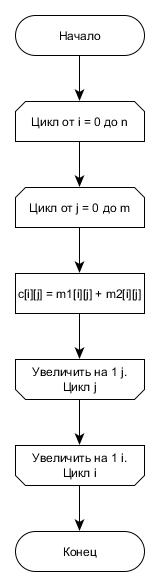
\includegraphics[scale=0.75]{classic.jpg}
    \caption{Схема алгоритма простого сложения матриц}
    \label{img:classic}
\end{figure}

\begin{figure}
    \centering
    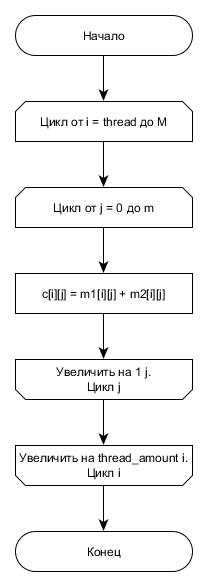
\includegraphics[scale=0.75]{parallel.jpg}
    \caption{Схема алгоритма параллельного сложения матриц}
    \label{img:parallel}
\end{figure}

\begin{figure}
    \centering
    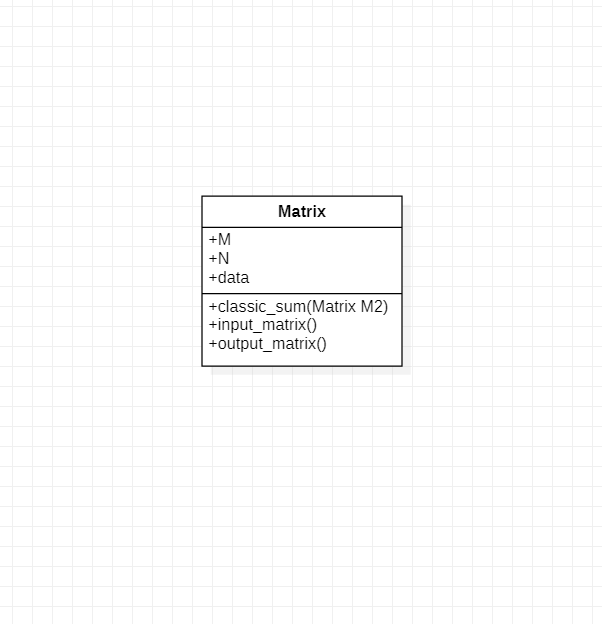
\includegraphics[scale=0.75]{diag_class.png}
    \caption{Диаграмма класса Matrix.}
    \label{img:diag}
\end{figure}

\section{Технологическая часть}

В данном разделе приведены требования к программному обеспечению, средства реализации и листинги кода.



\subsection{Средства реализации}


Для реализации программ был выбран язык программирования C++ [1]. Данный язык был выбран потому, что в нем присутствует инструментарий для замера процессорного времени и тестирования.

\subsection{Листинги кода}
\begin{lstlisting}[caption=Описание класса Matrix, label=list:canon, language={}]
template<class T>
class Matrix
{
public:
	int M;
	int N;
	vector<vector<T>> data;
	Matrix();
	Matrix(const Matrix<T>& M_);

	Matrix(int M_, int N_);


	Matrix<T> classic_sum(  Matrix<T>& M2);

	~Matrix<T>();

	Matrix<T>& input_matrix();

	void output_matrix();

};
\end{lstlisting}

\begin{lstlisting}[caption=Алгоритм простого сложения матриц, label=list:canon, language={}]
template <typename T>
Matrix<T> Matrix<T>::classic_sum( Matrix<T>& M2)
{
	Matrix<T> res(this->M, M2.N);
	for (int i = 0; i < res.M; i++)
	{
		for (int j = 0; j < res.N; j++)
		{
			res.data[i][j] = this->data[i][j] + M2.data[i][j];
		}
	}
	return res;

}
\end{lstlisting}

\begin{lstlisting}[caption=Алгоритм параллельного сложения матриц, label=list:vinograd, language={}]
template<class T>
void parallel_add(Matrix<T> matrix1, Matrix<T> matrix2, Matrix<T> &result, int thread, int threads_amount)
{

	for (int i = thread; i < result.M; i += threads_amount)
	{
		for (int j = 0; j < result.N; j++)
		{
			result.data[i] [j] = (matrix1.data[i][j] + matrix2.data[i][j]);
		}

	}
}
template<class T>
Matrix<T>  parallel_sum( Matrix<T> M1,  Matrix<T> M2, int threads_amount)
{
	Matrix<T> res(M1.M, M2.N);

	vector<thread> threads(threads_amount);

	for (int thread_ = 0; thread_ < threads_amount; thread_++)
	{
		threads[thread_] = thread(parallel_add<T>, M1, M2, std::ref(res), thread_, threads_amount);
	}

	for (int i = 0; i < threads_amount; i++)
	{
		threads[i].join();
	}

	return res;
}

\end{lstlisting}
\subsection{Тестирование функций}

В таблице \ref{tab:tests} приведены модульные тесты для функций сложения матриц выше перечисленными методами. Все тесты были пройдены успешно. \\

\begin{table}[hb]
    \caption{\centering Тестирование функций сложения матриц}
    \centering
    \begin{tabular}{ccc}
    Матрица 1 & Матрица 2 & Ожидаемый результат \\ \hline
    $\begin{pmatrix}
        1 & 2 & 3 \\
        4 & 5 & 6 \\
        7 & 8 & 9
    \end{pmatrix}$
    &$\begin{pmatrix}
        1 & 2 & 3 \\
        4 & 5 & 6 \\
        7 & 8 & 9
    \end{pmatrix}$
    &$\begin{pmatrix}
        2 & 4 & 6 \\
        8 & 10 & 12 \\
        14 & 16 & 18
    \end{pmatrix}$\\
    $\begin{pmatrix}
        1 & 2 \\
        4 & 5
    \end{pmatrix}$
    &$\begin{pmatrix}
        1 & 2 \\
        4 & 5
    \end{pmatrix}$
    &$\begin{pmatrix}
        2 & 4 \\
        8 & 10
    \end{pmatrix}$\\
    $\begin{pmatrix}
        8
    \end{pmatrix}$
    &$\begin{pmatrix}
        4
    \end{pmatrix}$
    &$\begin{pmatrix}
        12
    \end{pmatrix}$\\
    $\begin{pmatrix} 1 & 2 \end{pmatrix}$ & $\begin{pmatrix} 3 \end{pmatrix}$ & Сложение невозможно
    \end{tabular}
    \label{tab:tests}
    \end{table}

\subsection{Вывод}

Были разработаны и протестированы реализации алгоритмов: простой алгоритм сложения матриц, параллельный алгоритм сложения матриц.

\section{Исследовательская часть}
В данном разделе будут приведены результаты исследовательской деятельности - замеры процессорного времени работы алгоритмов и тестирование алгоритмов.

\subsection{Технические характеристики}

Технические характеристики электронно-вычислительнй машины, на которой выполнялось тестирование:

\begin{itemize}
    \item операционная система: Windows 10 64-bit;
    \item оперативная память: 8 гигабайт ;
    \item процессор: Intel i5 7th gen.
\end{itemize}


Тестирование проводилось на ноутбуке, включенном в сеть электропитания. Во время тестирования ноутбук был нагружен только встроенными приложениями окружения рабочего стола, окружением рабочего стола, а также непосредственно системой тестирования.

\subsection{Время выполнения алгоритмов}

Был проведен замер времени работы каждого из алгоритмов с помощью функции std::chrono::system clock::now. Эта функция замеряет процессорное время выполнения функции и усредняет его (проводится 20 замеров). В таблице \ref{tab:time_best} содержатся результаты исследований.

На рисунках \ref{img:plot_best}, \ref{img:plot_worst} демонстрируется зависимость времени выполнения конкретных реалзиаций алгоритмов сложения матриц от размера стороны квадратной матрицы и количества потоков соответственно. \\

\begin{table}[ht]
    \caption{\centering Время выполнения реализаций алгоритмов (в секундах) при количестве потоков 4.}
    \centering
    \begin{tabular}{|c|c|c|c|}
    \hline
    Размер & К      & П     \\ \hline
    100    & 0.021534 & 0.020617 \\ \hline
    200    & 0.040475 & 0.039583  \\ \hline
    500    & 0.518521  & 0.197411  \\ \hline
    1000    & 2.053641  & 0.519283  \\ \hline
 
    \end{tabular}
    \label{tab:time_best}
\end{table}

\begin{figure}
    \centering
    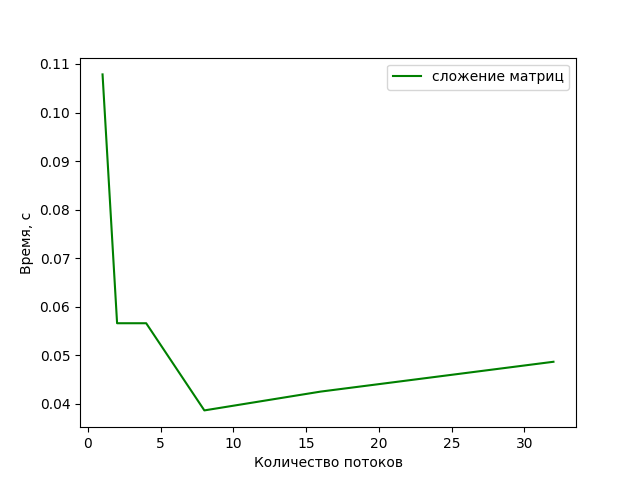
\includegraphics[scale=0.65]{ths.png}
    \caption{Зависимость времени выполнения алгоритмов от количества потоков при размере матрицы 1000 на 1000}
    \label{img:plot_best}
\end{figure}



\begin{figure}
    \centering
    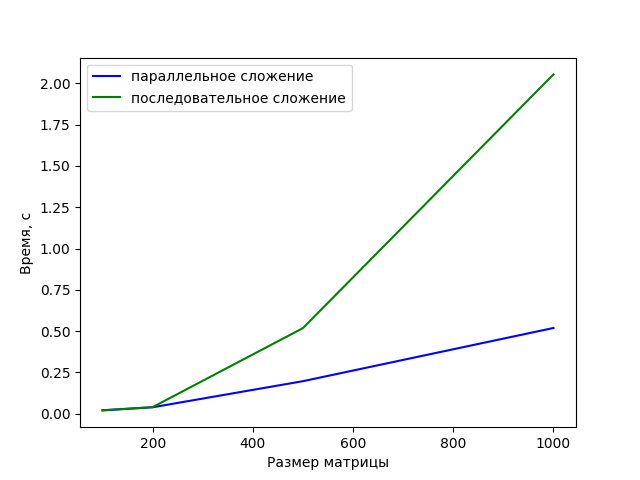
\includegraphics[scale=0.65]{sizes.png}
    \caption{Зависимость времени выполнения алгоритмов от размера стороны квадратной матрицы при количестве потоков 4}
    \label{img:plot_worst}
\end{figure}

\subsection{Вывод}

В данном разделе было произведено сравнение количества затраченного времени вышеизложенных алгоритмов.
Наиболее эффективным по времени алгоритмом при работе с матрицами больших размерностей (более 200 элементов) оказался параллельный алгоритм, работащий на 8 потоках.
При работе с матрицами малых размерностей (менее 200 элементов) стандартный алгоритм оказался более эффективным (~ в 4 раза в сравнении с 16 потоками), что связано с дополнительным затратами, которые необходимы при реализации многопоточности (создание потоков, реализация совместного доступа к ресурсам).


\anonsection{Заключение}


В ходе выполнения работы была достигнута цель выполнены все поставленные задачи:

\begin{itemize}
    \item реализовать классический алгоритм сложения матриц;
    \item реализовать параллельный алгоритм сложения матриц;
    \item сравнить их временные характеристики экспериментально;
    \item на основании проделанной работы сделать выводы.
\end{itemize}

Экспериментально были установлены различия в производительности различных алгоритмов сложения матриц. Параллельный алгоритм  имеет большую эффективность(при размерностях выше 200), нежели классический алгоритм сложения матриц. 
\anonsection{Список литература}

	\begin{enumerate}

		\item Т. Кормен, Ч. Лейзерсон, Р. Ривест, К. Штайн. Алгоритмы. Построение и анализ. Издательский дом ``Вильямс'', 2011. 823 - 869.
		\item Б. Страуструп. Язык программирования С++ . Addison-Wesley, 2000. 142 - 149.
		\item Г. Шилдт. С++. Полное руководство. СПб.: Наука и Техника, Издательский дом “Вильямс”, 2006. 621 - 693.
		\item Я. Галовиц. С++17 STL. Стандартная библиотека шаблонов. Серийная библиотека программиста, 2018. 91 - 123.
		\item Р. Седжвик. Фундаментальные алгоритмы С++. Diasoft, 2001. 42 - 69.

	\end{enumerate}

\end{document}
